\subsubsection{Principal Component Analysis}
\noindent
\par We substracted the mean accross voxels from our data in order to normalize the data.
We then apply the Single Value Decomposition (SVD) on the covariance matrix. The resulting
principal compoments are ordered according to the variance they explain in the data. 
The first principal component will be responsible for more variability than the second.
Our first approach is to vizualised the projection of the voxel by time matrix onto 
the principal components. In Figure \ref{fig:pcaa} we give then example of the run 1 
of the subject 1. 

\begin{figure}[H]
\begin{subfigure}{.5\textwidth}
    \centering
    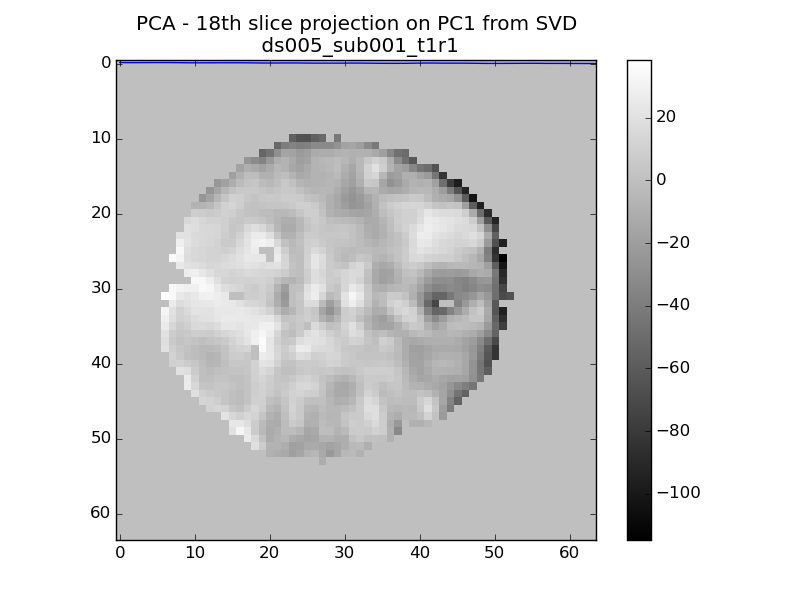
\includegraphics[width=.9\linewidth]{../fig/pca/ds005_sub001_t1r1_PC1.png}
    \caption{First principal component - PC1}
    \label{fig:pca1}
\end{subfigure}%
\begin{subfigure}{.5\textwidth}
    \centering
    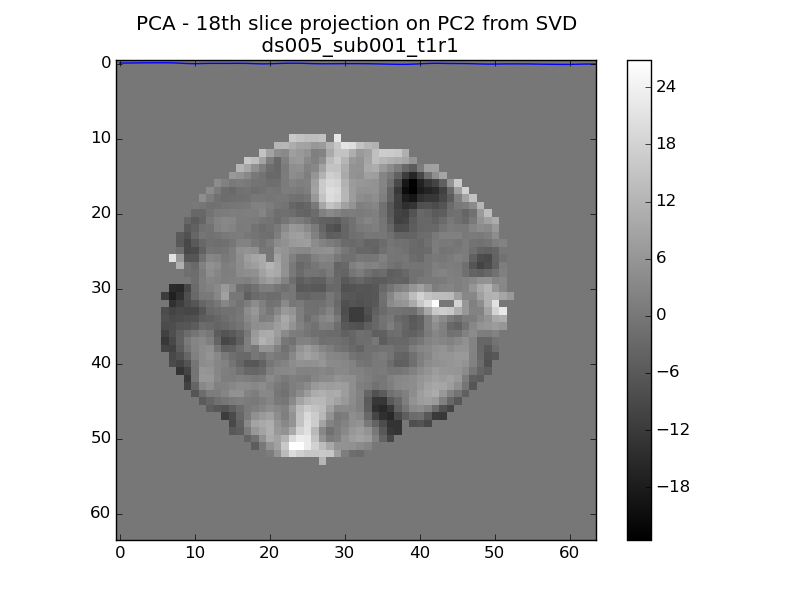
\includegraphics[width=.9\linewidth]{../fig/pca/ds005_sub001_t1r1_PC2.png}
    \caption{Second principal component = PC2}
    \label{fig:pca2}
\end{subfigure}
\caption{Brain data projected onto principal components of the data  - subject 1 - run 1}
\label{fig:pcaa}
\end{figure}

\noindent
The two images above, show that distinct localization of the voxels at the edges of the
brain, which suggests that they reflect brain anatomy rather than activation. 
We decided to remove these components by regression because they are likely to be 
related to noise from the scanner or the subject. 

\begin{figure}[H]
\begin{subfigure}{.5\textwidth}
    \centering
    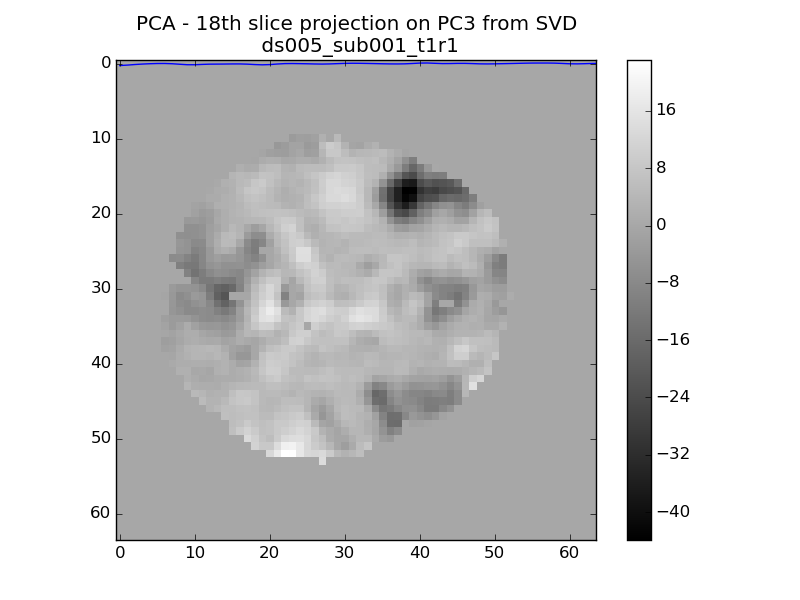
\includegraphics[width=.9\linewidth]{../fig/pca/ds005_sub001_t1r1_PC3.png}
    \caption{Third principal component - PC3}
    \label{fig:pca3}
\end{subfigure}%
\begin{subfigure}{.5\textwidth}
    \centering
    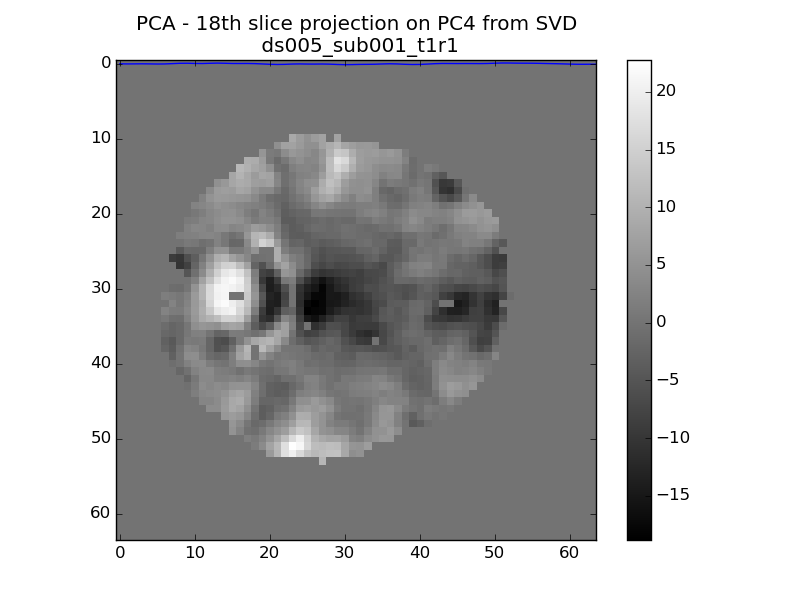
\includegraphics[width=.9\linewidth]{../fig/pca/ds005_sub001_t1r1_PC4.png}
    \caption{Fourth principal component = PC4}
    \label{fig:pca4}
\end{subfigure}
\caption{Brain data projected onto the princiipal components of the data- subject 1 - run 1}
\label{fig:pcab}
\end{figure}

\noindent
\par Contrary to the precedent cases, the above two images of of the data onto the 3rd 
and 4th principal component don't seem to reveal any random pattern. The projection on 
the 4th is even component show a darker area localized on the startium, region of interest
for our analysis.

\par A visual analysis is always difficult to perform to select the principal components. 
In order to determine how many principal components to include in our design matrix,
we plotted Variance Explained plots presented in the following sections.

\subsubsection{Variance explained} 
\noindent
\par In the Single Value Decomposition of the data, the the square roots of the 
singular values ordered from greatest to least along its diagonal. Each value 
indicates the variance of the component vector (time-course) along each principal component. 

\begin{figure}[H]
\begin{subfigure}{.5\textwidth}
    \centering
    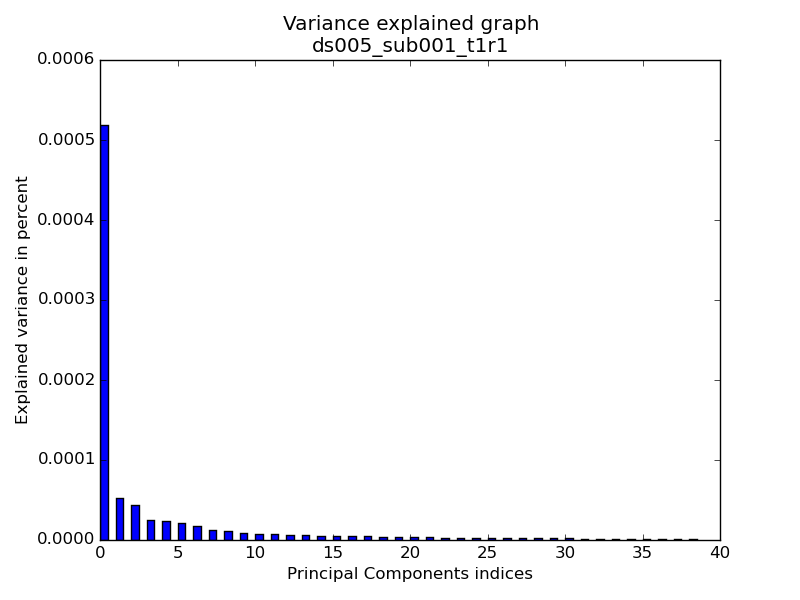
\includegraphics[width=.9\linewidth]{../fig/pca/ds005_sub001_t1r1_variance_explained.png}
    \caption{Subject 1}
    \label{fig:var1}
\end{subfigure}%
\begin{subfigure}{.5\textwidth}
    \centering
    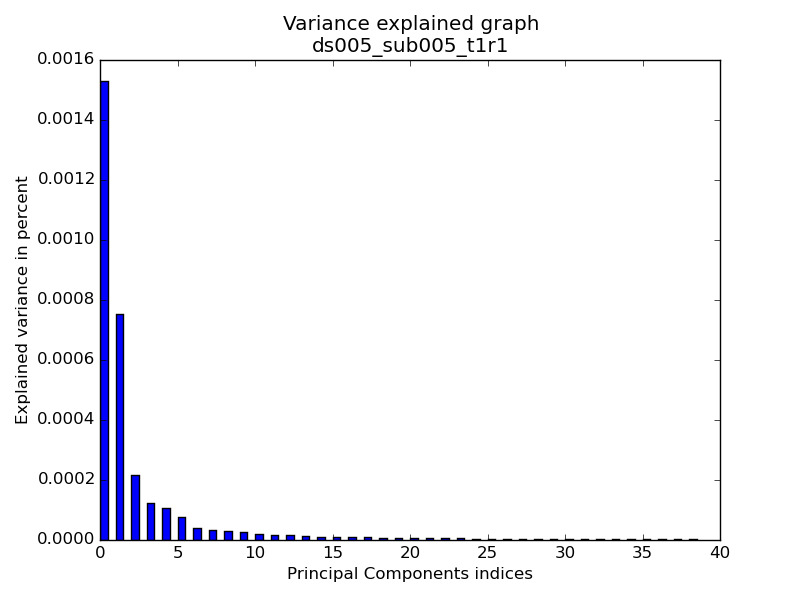
\includegraphics[width=.9\linewidth]{../fig/pca/ds005_sub005_t1r1_variance_explained.png}
    \caption{Subject 5}
    \label{fig:var2}
\end{subfigure}
\caption{Explained variance for the first [2-40] principal components of the data for subjects 1 and 5 - run 1 (the first component is not plotted for better clarity) }
\label{fig:vara}
\end{figure}

\noindent
\par In the Figure \ref{fig:vara}, we plotted the variance associated with each principal
components of the data. The first principal component accounts for more than 99percent of 
the overall variability. This is probably due to the high variability over time we did not
account for in the design of the PCA analysis. 
we decided to remove the first component from the following graph for better clarity.
In this particular case, the elbow shape of the graph makes a disctinction between the three first 
(the figure does not show the first principal component). Filtering out the first three principal 
components is justified here.

\subsubsection{Noise modeling results}
\noindent
\par We calculated the Mean Root Sum Square (MRSS) of the residuals of our different model.
For the run 1 of the subject 1, the mean of MRSS accross the voxels decreased from 23.89 
including only the drift terms to 7.32 with the inclusion of the three first principal 
components. We also performed the same modeling of the design matrix with the filtered data.
The mean MRSS resulting is 1.04 when we include the drift terms and 0.79 including the 
principal components.

\begin{figure}[H]
  \centering
  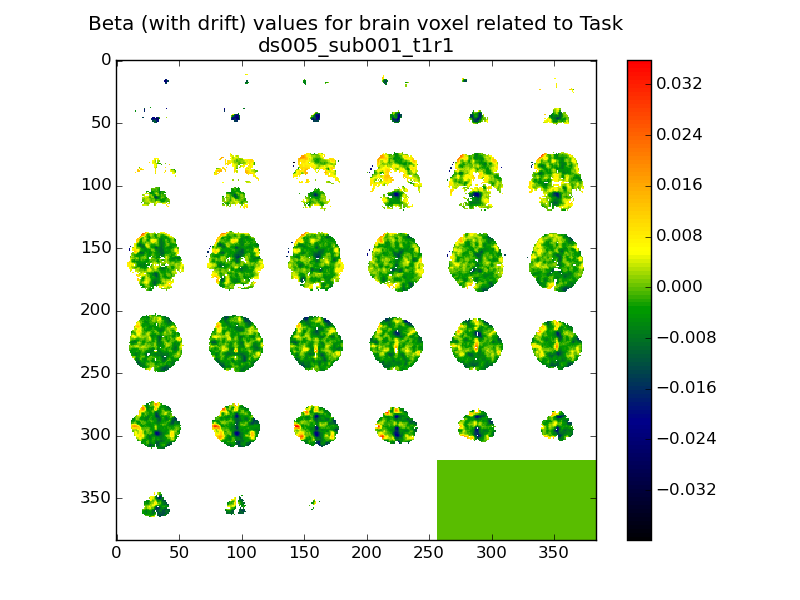
\includegraphics[scale=0.75]{../fig/mosaic/ds005_sub001_t1r1_withdrift_Task.png}
  \caption{Mean values of the Betas coefficients with drifts}
  \label{fig:betas1}
\end{figure}

\begin{figure}[H]
  \centering
  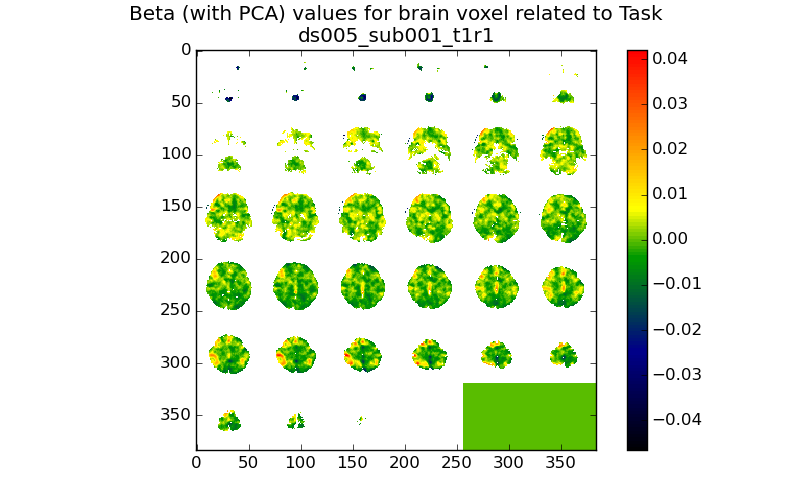
\includegraphics[scale=0.85]{../fig/mosaic/ds005_sub001_t1r1_withPCA_Task.png}
  \caption{Mean values of the Betas coefficients with PCs}
  \label{fig:betas2}
\end{figure}

\noindent
\par Betas coefficients of our linear model related to the brain activation with the task 
are plotted on the brain image in Figures \ref{fig:betas1} and \ref{fig:betas2}. We can see on both model 
(with or without the PC) we can localized the region of the brain related to the task 
activation thanks to the values of the betaghest the values are in red, the lowest in blue. 
From the journal article, we know the regions of interest are the inferior/middle frontal 
(see (100,200:400) and (150,0:300)), the ventral stratium (275, (150:400)) for example. 
Further analysis and statistical tests are needed to locate the activated voxels with task,
which is developped in the next section.

